\documentclass[border=5pt]{standalone}
\usepackage{tikz}
\usepackage{amsmath}
\usetikzlibrary{calc, positioning, arrows.meta, 3d}
\begin{document}
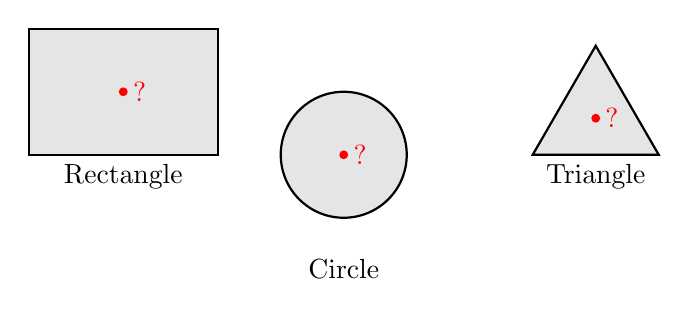
\begin{tikzpicture}[scale=0.8]
% Rectangle
\draw[thick, fill=gray!20] (0,0) rectangle (3,2);
\node[below] at (1.5,0) {Rectangle};
\fill[red] (1.5,1) circle (2pt) node[right] {?};

% Circle
\begin{scope}[shift={(5,0)}]
\draw[thick, fill=gray!20] (0,0) circle (1);
\node[below] at (0,-1.5) {Circle};
\fill[red] (0,0) circle (2pt) node[right] {?};
\end{scope}

% Equilateral triangle
\begin{scope}[shift={(8,0)}]
\draw[thick, fill=gray!20] (0,0) -- (2,0) -- (1,1.73) -- cycle;
\node[below] at (1,0) {Triangle};
\fill[red] (1,0.58) circle (2pt) node[right] {?};
\end{scope}
\end{tikzpicture}
\end{document}
